%%%%% Don't Make Changes Below Here %%%%%
\documentclass{article}\usepackage[utf8]{inputenc}\usepackage[margin=0.4cm,top=0.4cm,bottom=0.4cm]{geometry}\usepackage[usenames,dvipsnames,svgnames,table]{xcolor}
\usepackage{calligra}\usepackage{tikz}\usepackage{hyperref}\usetikzlibrary{matrix,fit,chains,calc,scopes}\usepackage{tcolorbox}\tcbuselibrary{skins}\tcbset{Baystyle/.style={sharp corners,enhanced,boxrule=6pt,colframe=orange,height=\textheight,width=\textwidth,borderline={8pt}{-11pt}{},}}\usepackage{amsmath,amssymb,amsthm,tikz,tkz-graph,color,chngpage,soul,hyperref,csquotes,graphicx,floatrow}\newcommand*{\QEDB}{\hfill\ensuremath{\square}}\newtheorem*{prop}{Proposition}\renewcommand{\theenumi}{\alph{enumi}}\usepackage[shortlabels]{enumitem}\usetikzlibrary{matrix,calc}\MakeOuterQuote{"}\newtheorem{theorem}{Theorem} \usetikzlibrary{shapes} \usepackage{lipsum}\usepackage{tabularx,ragged2e,booktabs,caption}\tcbuselibrary{breakable}\newenvironment{yframed}{\begin{tcolorbox}[breakable,colback=gray!3,title after break={\textit{\color{red}Solution (cont.)}},colbacktitle=gray!3, coltitle=black,titlerule=-1pt] }{\end{tcolorbox}}\newtcolorbox{mybox}{colback=black!15!white, colframe=white,arc=12pt}\newtcolorbox{myboxot}{colback=green!15!white, colframe=white,arc=12pt,width=110pt, height=27pt}\newtcbox{\mylib}{enhanced,boxrule=0pt,top=0mm,bottom=0mm,right=0mm,left=4mm,arc=4pt,boxsep=9pt,before upper={\vphantom{dlg}},colframe=green!50!black,coltext=green!25!black,colback=green!10!white,overlay={\begin{tcbclipinterior}\fill[green!75!blue!50!white] (frame.south west)rectangle node[text=white,font=\sffamily\bfseries\tiny,rotate=90] {Problem} ([xshift=4mm]frame.north west);\end{tcbclipinterior}}}\newtcbox{\mylibot}{enhanced,boxrule=0pt,top=0mm,bottom=0mm,right=0mm,arc=4pt,boxsep=9pt,before upper={\vphantom{dlg}},colframe=green!50!black,coltext=green!25!black,colback=green!10!white,overlay={\begin{tcbclipinterior}\fill[red!75!blue!50!white] (frame.south west)rectangle node[text=white,font=\sffamily\bfseries\tiny,rotate=90] {Other} ([xshift=4mm]frame.north west);\end{tcbclipinterior}}}
\def\Title{\begin{tcolorbox}[Baystyle,]{\begin{center}\vspace*{0.14\textheight}
{\rule{\textwidth}{1.6pt}\vspace*{-\baselineskip}\vspace*{2pt}}
\rule{\textwidth}{0.4pt}\\[0.2\baselineskip]{\fontsize{45}{45}\scshape CS 189: Introduction to Machine Learning \\[0.2\baselineskip] \calligra Spring 2018 \\[0.2\baselineskip]}
{\rule{\textwidth}{0.4pt}\vspace*{-\baselineskip}\vspace{3.2pt}}
\rule{\textwidth}{1.6pt}\\[\baselineskip]\vspace{0.05\textheight}{{\fontsize{45}{45}\scshape$\bullet$\\ {Homework 3}\\\vspace*{0.01\textheight} }{{\fontsize{18}{18}\scshape{Due on Friday, February 10th, 2018 at 10pm\\}}}\fontsize{45}{45}\scshape$\bullet$  \\}\vspace*{0.1\textheight}{\fontsize{12}{12}\calligra Solutions by\\}{\fontsize{28}{28}\scshape \Name \\}\vspace*{0.01\textheight}{\fontsize{12}{12}\scshape \SID} \\\vspace*{0.05\textheight}{\fontsize{12}{12}\calligra In collaboration with\\}\vspace*{0.01\textheight}{\fontsize{12}{12}\scshape \Collabs} \\\vspace*{0.05\textheight}\end{center}}\end{tcolorbox}\newgeometry{margin=0.75in}}\def\BeginSolution{\begin{yframed}\textbf{\color{red}Solution }}\def\EndSolution{\end{yframed}}
\usepackage{algorithm}\usepackage[noend]{algpseudocode}\makeatletter\def\BState{\State\hskip-\ALG@thistlm}\makeatother\def\T{\indent}\def\star{\bigstar}
\usetikzlibrary{arrows}
\usepackage[mathscr]{euscript}
\usepackage[T1]{fontenc}
\DeclareSymbolFont{rsfs}{U}{rsfs}{m}{n}
\DeclareSymbolFontAlphabet{\mathscrsfs}{rsfs}
\newcommand\tab[1][1cm]{\hspace*{#1}}
\hypersetup{colorlinks=true,urlcolor=blue}
\newtheorem{lemma}[theorem]{Lemma}
\newcommand{\norm}[1]{\left\lVert#1\right\rVert}
%%%%% Don't Make Changes Above Here %%%%%

%%%%% Template Begins Here %%%%%

\def\Name{Firstname Lastname}  % Your name
\def\SID{Student ID}  % Your student ID number
\def\Collabs{None} % Your collaborators here with a comma between each person's name. Write None if no collaborators. Don't leave blank.


\pagestyle{empty}
\begin{document}
\Title
\clearpage

%%%% Problem 1 Starts Here %%%%
\vspace{-2mm}\noindent\begin{mybox}{\begin{center}\textbf{\color{black}Problem 1: Getting Started}\end{center}}\end{mybox}\vspace{-2mm}
\vspace{10pt}
\noindent \textbf{Read through this page carefully.} You may typeset your homework in latex or submit neatly handwritten/scanned solutions. Please start each question on a new page. Deliverables:
\begin{enumerate}[1.]
\item Submit a PDF of your writeup, \textbf{with an appendix for your code}, to assignment on Gradescope, ``HW3 Write-Up''. If there are graphs, include those graphs in the correct sections. Do not simply reference your appendix.
\item If there is code, submit all code needed to reproduce your results, ``HW3 Code''.
\item If there is a test set, submit your test set evaluation results, ``HW3 Test Set''.
\end{enumerate}
After you've submitted your homework, watch out for the self-grade form.
\begin{enumerate}
\item Who else did you you work with on this homework? In case of course events, just describe the group. How did you work on this homework? Any comments about the homework?
\BeginSolution
%1a

\EndSolution
\item Please copy the following statement and sign next to it. We just want to make it \textit{extra} clear so that no one inadvertently cheats.

\textit{I certify that all solutions are entirely in my words and that I have not looked at another student's solutions. I have credited all external sources in this write up.}
\BeginSolution
%1b

\EndSolution
\end{enumerate}
%%%% Problem 1 Ends Here %%%%
\clearpage

%%%% Problem 2 Starts Here %%%%
\vspace{-2mm}\noindent\begin{mybox}{\begin{center}\textbf{\color{black}Problem 2: Probabilistic Model of Linear Regression}\end{center}}\end{mybox}\vspace{-2mm}
\vspace{10pt}
\noindent Both ordinary least squares and ridge regression have interpretations from a probabilistic standpoint. In particular, assuming a generative model for our data and a particular noise distribution, we will derive least squares and ridge regression as the maximum likelihood and maximum {\em a-posteriori} parameter estimates, respectively. This problem will walk you through a few steps to do that. (Along with some side digressions to make sure you get a better intuition for ML and MAP estimation.)  
\begin{enumerate}
\item Assume that $X$ and $Y$ are both one-dimensional random variables, i.e. $X, Y \in \mathbb{R}$. Assume an affine model between $X$ and $Y$: $Y=Xw_1+w_0+Z$, where $w_1, w_0 \in \mathbb{R}$, and $Z \sim N(0,1)$ is a standard normal (Gaussian) random variable.  Assume $w_1, w_0$ are fixed parameters (i.e., they are not random).  {\bf What is the conditional distribution of $Y$ given $X$?}
\BeginSolution
%2a

\EndSolution
\item Given $n$ points of training data $\{(X_1,Y_1),(X_2,Y_2),\ldots, (X_n,Y_n)\}$ generated in an iid fashion by the probabilistic setting in the previous part, {\bf derive the maximum likelihood estimator for $w_1,w_0$ from this training data.} 
\BeginSolution
%2b

\EndSolution
\item Now, consider a different generative model. Let $Y=Xw+Z$, where $Z \sim U[-0.5,0.5]$ is a continuous random variable uniformly distributed between $-0.5$ and $0.5$.  Again assume that $w$ is a fixed parameter. {\bf What is the conditional distribution of $Y$ given $X$?} 
\BeginSolution
%2c

\EndSolution
\item Given $n$ points of training data $\{(X_1,Y_1),(X_2,Y_2),\cdots, (X_n,Y_n)\}$ generated in an i.i.d. fashion in the setting of the part (c) {\bf derive a maximum likelihood estimator of $w$.} Assume that $X_i > 0$ for all $i = 1, \ldots, n$. (Note that MLE for this case need not be unique;  but you are required to report only one particular estimate.)
\BeginSolution
%2d

\EndSolution
\item Take the model $Y=Xw +Z$, where $Z \sim U[-0.5,0.5]$. {\bf Use a computer to simulate $n$ training samples $\{(X_1,Y_1),(X_2,Y_2),\cdots, (X_n,Y_n)\}$ and illustrate what the likelihood of the data looks like as a function of $w$ after $n=5, 25, 125, 625$ training samples. Qualitatively describe what is happening as $n$ gets large.}  
\vspace{4pt}

\noindent (You may use the starter code. Note that you have considerable design freedom in this problem part. You get to choose how you draw the $X_i$ as well as what true value $w$ you want to illustrate. You have total freedom in using additional python libraries for this problem part. No restrictions.) 
\BeginSolution
%2e

\EndSolution
\item (One-dimensional Ridge Regression) Now, let us return to the case of Gaussian noise. Given $n$ points of training data $\{(X_1,Y_1),(X_2,Y_2),\cdots, (X_n,Y_n)\}$ generated according to $Y_i=X_i W+Z_i$, where $Z_i \sim N(0,1)$ are iid standard normal random variables. Assume $W \sim N(0,\sigma^2)$ is also a standard normal and is independent of both the $Z_i$'s and the $X_i$'s. {\bf Use Bayes' Theorem to derive the posterior distribution of $W$ given the training data. What is the mean of the posterior distribution of $W$ given the data?}
\vspace{4pt}

\noindent Hint: Compute the posterior up-to proportionality and try to identify the distribution by completing the square.
\BeginSolution
%2f

\EndSolution
\item Consider $n$ training data points $\{(\mathbf{x}_1,Y_1),(\mathbf{x}_2,Y_2),\cdots, (\mathbf{x}_n,Y_n)\}$ generated according to $Y_i=\mathbf w^\top \mathbf{x}_i+Z_i$ where $Y_i\in\mathbb{R}, \mathbf{w}, \mathbf{x}_i \in\mathbb{R}^d$ with $\mathbf w$ fixed, and $Z_i \sim N(0,1)$ iid standard normal random variables.  {\bf Argue why the maximum likelihood estimator for $\mathbf w$ is the solution to a least squares problem.} 
\BeginSolution
%2g

\EndSolution
\item (Multi-dimensional ridge regression) Consider the setup of the previous part: $Y_i= \mathbf{W}^\top \mathbf{x}_i+Z_i$, where $Y_i\in\mathbb{R}, \mathbf{W}, \mathbf{x}_i \in\mathbb{R}^d$, and $Z_i \sim N(0,1)$ iid standard normal random variables. Now we treat $\mathbf{W}$ as a random vector and assume a prior knowledge about its distribution. In particular, we use the prior information that the random variables $W_j$ are i.i.d. $\sim N(0,\sigma^2)$ for $j=1,2,\ldots,d$. {\bf Derive the posterior distribution of $\mathbf{W}$ given all the $\mathbf{x}_i,Y_i$ pairs. What is the mean of the posterior distribution of the random vector $\mathbf{W}$?} 
\vspace{4pt}

\noindent Hint: Use hints from part (f) and the following identities: For $\mathbf{X} = \begin{bmatrix}  \mathbf {x}_1^\top  \\ \vdots \\ \mathbf{x}_n^\top \end{bmatrix} $ and $\mathbf{Y} = \begin{bmatrix}  Y_1 \\ \vdots \\ Y_n \end{bmatrix}$ we have $\mathbf{X}^\top \mathbf{X} = \sum_{i=1}^n \mathbf{x}_i\mathbf{x}_i^\top $ and $\mathbf{X}^T \mathbf{Y} = \sum_{i=1}^n \mathbf{x}_i Y_i$.
\BeginSolution
%2h

\EndSolution
\item Consider $d=2$ and the setting of the previous part. {\bf Use a computer to simulate and illustrate what the {\em a-posteriori} probability looks like for the $W$ model parameter space after $n=5, 25, 125$ training samples for different values of $\sigma^2$. } 
\vspace{4pt}

\noindent (Again, you may use the starter code. And like problem (e), there are no restrictions for using additional python libraries for this part as well.)  
\BeginSolution
%2i

\EndSolution
\end{enumerate}
%%%% Problem 2 Ends Here %%%%
\clearpage

%%%% Problem 3 Starts Here %%%%
\vspace{-2mm}\noindent\begin{mybox}{\begin{center}\textbf{\color{black}Problem 3: Simple Bias-Variance Tradeoff}\end{center}}\end{mybox}\vspace{-2mm}
\vspace{10pt}
\noindent Consider a random variable $X$, which has unknown mean $\mu$ and unknown variance $\sigma^2$. Given $n$ iid realizations of training samples $X_1=x_1, X_2=x_2, \ldots, X_n=x_n$ from the random variable, we wish to estimate the mean of $X$. We will call our estimate of $X$ the random variable $\hat{X}$, which has mean $\hat{\mu}$. There are a few ways we can estimate $\mu$ given the realizations of the $n$ samples:
\begin{enumerate}[1.]\item Average the $n$ samples: $\displaystyle \frac{x_1+x_2+\ldots+x_n}{n}$.\item Average the $n$ samples and one sample of $0$: $\displaystyle\frac{x_1+x_2+\ldots+x_n}{n+1}$.\item Average the $n$ samples and $n_0$ samples of $0$: $\displaystyle\frac{x_1+x_2+\ldots+x_n}{n+n_0}$.\item Ignore the samples: just return $0$.\end{enumerate} \noindent In the parts of this question, we will measure the \emph{bias} and \emph{variance} of each of our estimators. The \emph{bias} is defined as $$\mathbb{E}[\hat{X} - \mu]$$ and the $\emph{variance}$ is defined as $$\text{Var}[\hat{X}]$$
\begin{enumerate}
\item \textbf{What is the bias of each of the four estimators above?}
\BeginSolution
%3a

\EndSolution
\item \textbf{What is the variance of each of the four estimators above?}
\BeginSolution
%3b

\EndSolution
\item Suppose we have constructed an estimator $\hat X$ from some samples of $X$. We now want to know how well $\hat X$ estimates a fresh (new) sample of $X$. Denote this fresh sample by $X'$. Note that $X'$ is an i.i.d. copy of the random variable $X$. \textbf{Derive a general expression for the expected squared error $\mathbb{E}[(\hat{X} - X')^2] $ in terms of $\sigma^2$ and the bias and variance of the estimator $\hat X$. Similarly, derive an expression for the expected squared error $\mathbb{E}[(\hat{X} - \mu)^2]$. Compare the two expressions and comment on the differences between them, if any.}
\BeginSolution
%3c

\EndSolution
\item It is a common mistake to assume that an unbiased estimator is always "best". Let's explore this a bit further. \textbf{Compute the expected squared error for each of the estimators above.}
\BeginSolution
%3d

\EndSolution
\item textbf{Demonstrate that the four estimators are each just special cases of the third estimator, but with different instantiations of the hyperparameter $n_0$}.
\BeginSolution
%3e

\EndSolution
\item \textbf{What happens to bias as $n_0$ increases? What happens to variance as $n_0$ increases?}
\BeginSolution
%3f

\EndSolution
\item Say that $n_0 = \alpha n$. \textbf{Find the setting for $\alpha$ that would minimize the expected total error, assuming you secretly knew $\mu$ and $\sigma$.} Your answer will depend on $\sigma$, $\mu$, and $n$.
\BeginSolution
%3g

\EndSolution
\item For this part, let's assume that we had some reason to believe that $\mu$ \emph{should be small} (close to $0$) and $\sigma$ \emph{should be large}. In this case, \textbf{what happens to the expression in the previous part?}
\BeginSolution
%3h

\EndSolution
\item In the previous part, we assumed there was reason to believe that $\mu$ \emph{should be small}. Now let's assume that we have reason to believe that $\mu$ is not necessarily small, but \emph{should be close to some fixed value} $\mu_0$. \textbf{In terms of $X$ and $\mu_0$, how can we define a new random variable $X'$ such that $X'$ is expected to have a small mean? Compute the mean and variance of this new random variable.}
\BeginSolution
%3i

\EndSolution
\item Draw a connection between $\alpha$ in this problem and the regularization parameter $\lambda$ in the ridge-regression version of least-squares. \textbf{What does this problem suggest about choosing a regularization coefficient and handling our data-sets so that regularization is most effective}? This is an open-ended question, so do not get too hung up on it.
\BeginSolution
%3j

\EndSolution
\end{enumerate}
%%%% Problem 3 Ends Here %%%%
\clearpage

%%%% Problem 4 Starts Here %%%%
\vspace{-2mm}\noindent\begin{mybox}{\begin{center}\textbf{\color{black}Problem 4: Estimation and approximation in linear regression}\end{center}}\end{mybox}\vspace{-2mm}
\vspace{10pt}
\noindent In typical applications, we are dealing with data generated by an \emph{unknown} function (with some noise), and our goal is to estimate this function. So far we used linear and polynomial regressions. In this problem we will explore the quality of polynomial regressions when the true function is not polynomial.
\vspace{4pt}

\noindent Suppose we are given a full column rank feature matrix $\mathbf{X} \in \mathbb{R}^{n \times d}$ and an observation vector $\mathbf{y}\in \mathbb{R}^n$. Let the vector $\mathbf y$ represent the noisy measurement of a true signal $\mathbf{y}^*$: \begin{align}  \mathbf{y} = {\mathbf{y}^*} + \mathbf{z}  \label{eq:model} \end{align} with $\mathbf{z} \in \mathbb{R}^n$ representing the random noise in the observation $\mathbf{y}$, where $z_j \sim \mathcal{N}(0,\sigma^2)$ are i.i.d. We define the vectors $\mathbf{w}^*$ and $\hat{\mathbf{w}}$ as follows: \begin{align*} \mathbf{w}^* = \arg\min_{\mathbf {w}} \| \mathbf {y}^* - \mathbf{X} \mathbf {w} \|_2^2\quad\quad\text{and}\quad\quad \hat{\mathbf {w}} = \arg\min_{\mathbf {w}} \| \mathbf{y} - \mathbf{X} \mathbf{w}\|_2^2. \end{align*} Observe that for a given true signal $\mathbf{y}^*$ the vector $\mathbf{w}^*$ is fixed, but the vector $\hat{\mathbf w}$ is a random variable since it is a function of the random noise $\mathbf z$. Note that the vector $\mathbf{X}\mathbf{w}^*$ is the best linear fit of the true signal $\mathbf{y}^*$ in the column space of $\mathbf{X}$. Similarly, the vector $\mathbf{X} \hat{\mathbf{w}}$ is the best linear fit of the observed noisy signal $\mathbf{y}$ in the column space of $\mathbf{X}$.
\vspace{4pt}

\noindent After obtaining $\hat{\mathbf{w}}$, we would like to bound the error $\| \mathbf{X} \hat{\mathbf{w}} - \mathbf{y}^*\|_2^2$, which is the \emph{prediction error} incurred based on the specific $n$ training samples. In this problem we will see how to get a good estimate of this prediction error. When using polynomial features, we will also learn how to decide the degree of the polynomial when trying to fit a noisy set of observations from a smooth function.
\vspace{4pt}

\noindent {\bf Remark}: You can use the closed form solution for OLS and results from Discussion 3 for all parts of this problem. For parts (a) to (c), assume that the feature matrix $\mathbf{X}$ and the true signal vector $\mathbf{y}^*$ are fixed (and not random). Furthermore, in all parts the expectation is taken over the randomness in the noise vector $\mathbf{z}$. 
\begin{enumerate}
\item {\bf Show that} $\mathbb{E}[\hat{\mathbf{w}}] = \mathbf{w}^*$ and use this fact to {\bf show that} \begin{align*}   \mathbb{E}\left[\| \mathbf{y}^* - \mathbf{X} \hat{\mathbf{w}} \|_2^2\right]   = \| \mathbf y^* - \mathbb{E}[\mathbf X \hat{\mathbf w}] \|_2^2 +   \mathbb{E}\left[\| \mathbf X \hat{\mathbf w}  - \mathbb{E}[\mathbf X \hat{\mathbf w}\|_2^2\right]. \end{align*} Note that the above decomposition of the squared error corresponds to the sum of bias-squared and the variance of our estimator $\mathbf X \hat{\mathbf w}$.
\BeginSolution
%4a

\EndSolution
\item Recall that if $\mathbf{v} \sim \mathcal{N}(\mathbf{0}, \Sigma)$, where $\Sigma \in \mathbb{R}^{(d \times d)}$ is the covariance matrix, then for any matrix $A \in \mathbb{R}^{k \times d}$, we have $\mathbf{A}\mathbf{v} \sim \mathcal{N}(\mathbf{0}, \mathbf{A}\Sigma\mathbf{A}^T)$. Use this fact to {\bf show that} the distribution of the vector $\hat{\mathbf{w}}$ is given by $$\hat{\mathbf{w}} \sim \mathcal{N}(\mathbf{w}^*, \sigma^2(\mathbf{X}^\top \mathbf{X})^{-1})$$
\BeginSolution
%4b

\EndSolution
\item Use part (b) to {\bf show that} $$\frac{1}{n} \mathbb{E} \left[ \| \mathbf{X} \hat{\mathbf{w}} - \mathbf{X} \mathbf w^* \|_2^2 \right] = \sigma^2 \frac{d}{n}$$
\vspace{4pt}

\noindent Hint: The trace trick: ${\mathrm{trace}}(AB) = {\mathrm{trace}}(BA)$, might be useful.
\BeginSolution
%4c

\EndSolution
\item Assume the underlying model is a noisy linear model with scalar samples $\{\alpha_i, y_i\}_{i=1}^n$, i.e. $y_i = w_1 \alpha_i + w_0 + z_i$. We construct matrix $\mathbf{X}$ by using $D+1$ polynomial features $\mathbf{P}_D(\alpha_i) = [1, \alpha_i, \ldots, \alpha_i^D]^\top$ of the \emph{distinct} sampling points $\{\alpha_i\}_{i=1}^n$. For any $D \geq 1$, compare with model~\eqref{eq:model} and {\bf compute $\mathbf{w}^*$ for this case. Also compute the bias ($\Vert \mathbf{y}^* - \mathbf{X} \mathbf{w}^*\Vert_2$) for this case.} Using the previous parts of this problem, {\bf compute the number of samples $n$ required to ensure that the average expected prediction squared error is bounded by $\epsilon$?} Your answer should be expressed as a function of $D$, $\sigma^2$, and $\epsilon$.
\vspace{4pt}

\noindent {\bf Conclude that as we increase model complexity, we require a proportionally larger number of samples for accurate prediction.}
\BeginSolution
%4d

\EndSolution
\item Simulate the problem from part (d) for yourself. Set $w_1 = 1$, $w_0 = 1$, and sample $n$ points $\{\alpha_i\}_{i=1}^n$ uniformly from the interval $[-1,1]$. Generate $y_i = w_1 \alpha_i + w_0 + z_i$ with $z_i$ representing standard Gaussian noise.
\vspace{4pt}

\noindent {\bf Fit a $D$ degree polynomial to this data and show how the average error $\frac{1}{n} \| \mathbf{X} \hat{\mathbf{w}} - \mathbf{y}^* \|_2^2$ scales as a function of both $D$ and $n$.}
\vspace{4pt}

\noindent You may show separate plots for the two scalings. It may also be helpful to average over multiple realizations of the noise (or to plot point clouds) so that you obtain smooth curves.
\vspace{4pt}

\noindent (For this part, the libraries \texttt{numpy.random} and \texttt{numpy.polyfit} might be useful. You are free to use any and all python libraries.)
\BeginSolution
%4e

\EndSolution
\item Assume that the underlying model is the noisy exponential function with scalar samples $\{\alpha_i, y_i\}_{i=1}^n$ where  $y_i = e^{\alpha_i} + z_i$ with  \emph{distinct} sampling points $\{\alpha_i\}_{i=1}^n$, in the interval $[-4,3]$ and i.i.d. Gaussian noise $z_i \sim \mathcal{N}(0, 1)$. We again construct matrix $\mathbf{X}$ by using $D+1$ polynomial features $[1, \alpha_i, \ldots, \alpha_i^D]^\top$ and use linear regression to fit the observations. Recall, the definitions of the bias and variance of the OLS estimator from part (a) and {\bf show that for a fixed $n$, as the degree $D$ of the polynomial increases: (1) the bias decreases and (2) the variance increases}. Use the values you derived for bias and variance and {\bf show that for the prediction error, the optimal choice of $D$ is given by $\mathcal{O}(\log n/\log\log n)$}.
\vspace{4pt}

\noindent Hint: You can directly use previous parts of this problem, Discussion 3 and Problem 4 of HW 2. You may assume that $n$ and $D$ are large for approximation purposes.
\BeginSolution
%4f

\EndSolution
\item Simulate the problem in part (f) yourself. Sample $n$ points $\{\alpha_i\}_{i=1}^n$ uniformly from the interval $[-4, 3]$. Generate $y_i = e^{\alpha_i} + z_i$ with $z_i$ representing standard Gaussian noise. {\bf Fit a $D$ degree polynomial to this data and show how the average error $\frac{1}{n} \| \mathbf{X} \hat{\mathbf{w}} - \mathbf{y}^* \|_2^2$ scales as a function of both $D$ and $n$.} You may show separate plots for the two scalings. For scaling with $D$, choose $n = 120$. It may also be helpful to average over multiple realizations of the noise (or to plot point clouds) so that you obtain smooth curves. (For this part, the libraries \texttt{numpy.random} and \texttt{numpy.polyfit} might be useful and you are free to use any and all python libraries.)
\BeginSolution
%4g

\EndSolution
\item Comment on the differences in plots obtained in part (e) and part (g).
\BeginSolution
%4h

\EndSolution
\end{enumerate}
%%%% Problem 4 Ends Here %%%%
\clearpage

%%%% Problem 5 Starts Here %%%%
\vspace{-2mm}\noindent\begin{mybox}{\begin{center}\textbf{\color{black}Problem 5: Robotic Learning of Controls from Demonstrations and Images}\end{center}}\end{mybox}\vspace{-2mm}
\vspace{10pt}
\noindent Huey, a home robot, is learning to retrieve objects from a cupboard, as shown in Fig.~\ref{fig:robot}. The goal is to push obstacle objects out of the way to expose a goal object.  Huey's robot trainer, Anne, provides demonstrations via tele-operation. When tele-operating the robot, Anne can look at the images captured by the robot and provide controls to Huey remotely.
\vspace{4pt}

\noindent During a demonstration, Huey records the RGB images of the scene for each timestep, $x_0,x_1,...,x_{n}$, where $x_i \in \mathbb{R}^{30\times 30\times 3}$ and the controls for his body, $u_0,u_1,\ldots,u_{n}$, where $u_i \in \mathbb{R}^3$. The controls correspond to making small changes in the 3D pose (i.e. translation and rotation) of his body. Examples of the data are shown in the figure. 
\vspace{4pt}

\noindent Under an assumption (sometimes called the Markovian assumption) that all that matters for the current control is the current image, Huey can try to learn a linear \emph{policy} $\pi$ (where $\pi \in \mathbb{R}^{2700\times 3}$) which linearly maps image states to controls (i.e. $\pi^\top x =u$). We will now explore how Huey can recover this policy using linear regression. Note please use {\bf numpy} and {\bf numpy.linalg} to complete this assignment. 
\vspace{4pt}

\noindent \begin{figure}[h!] \begin{center} 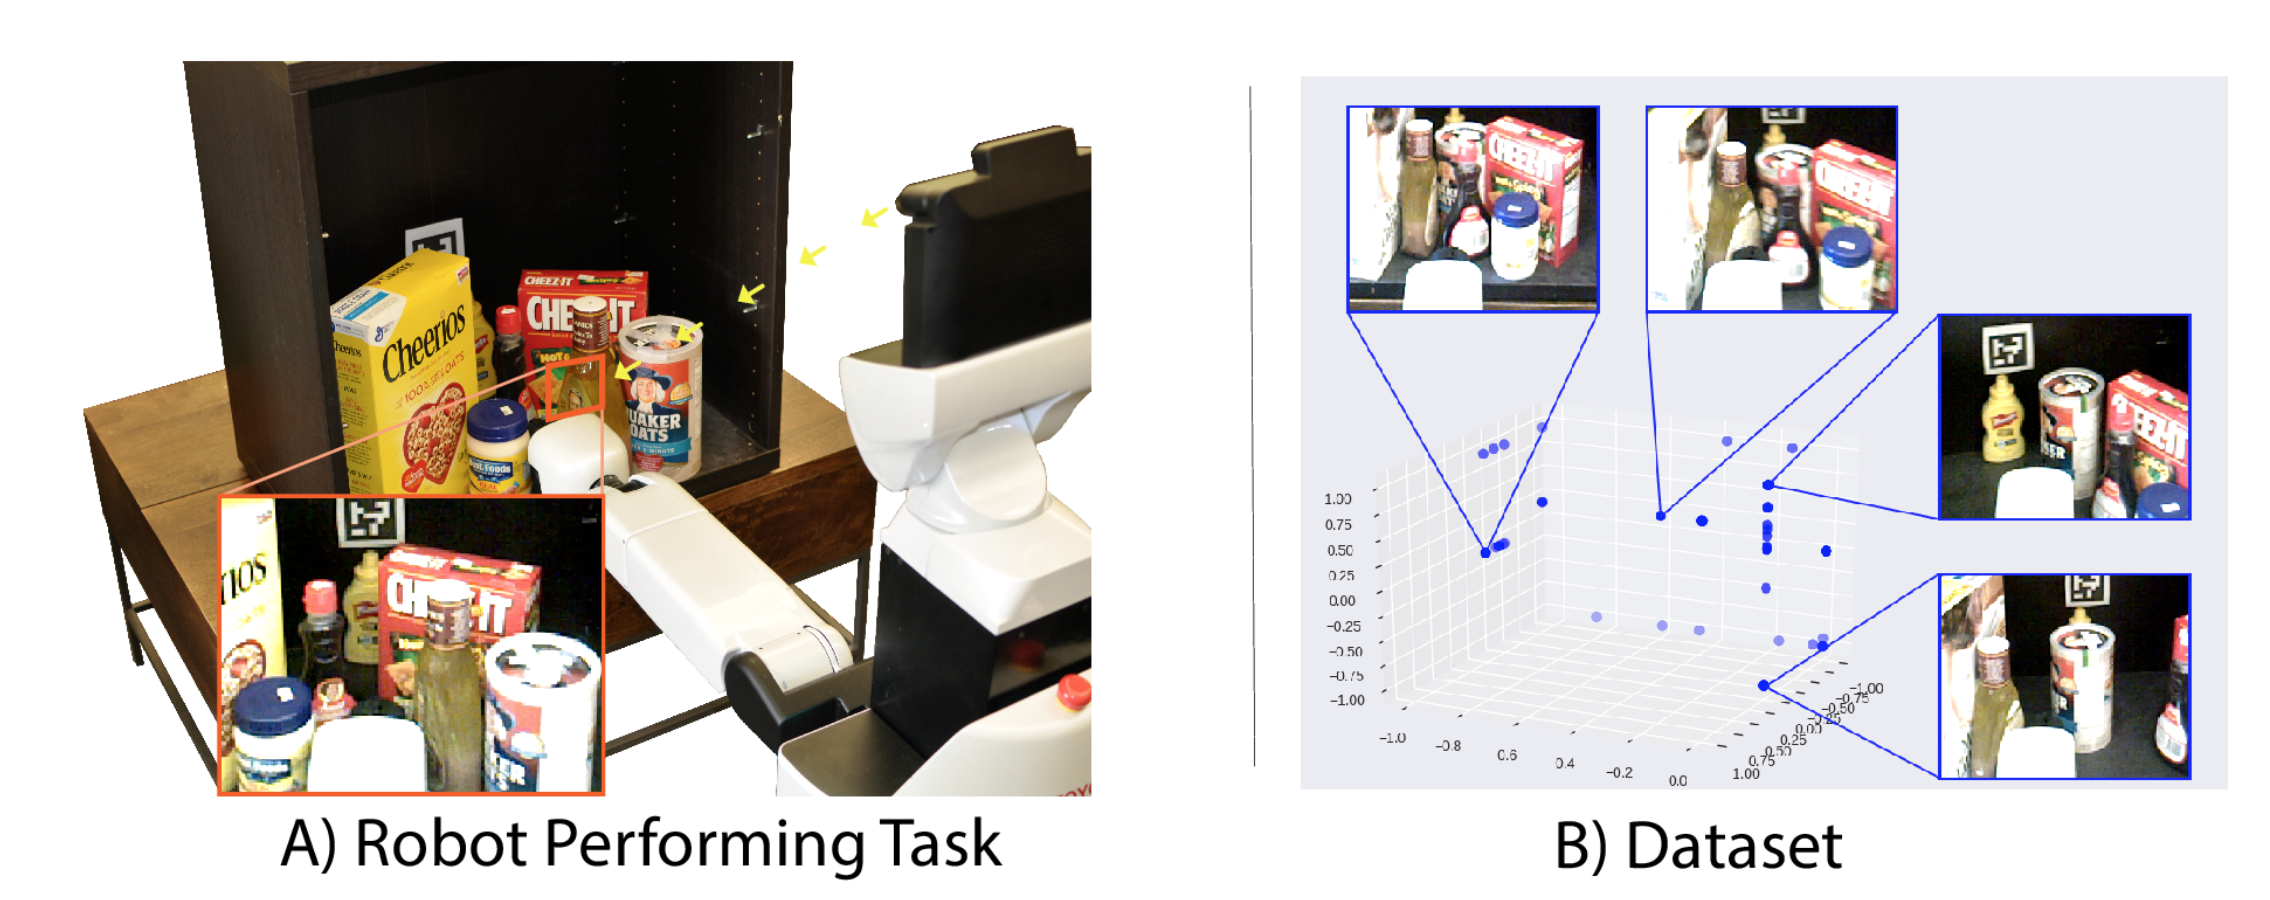
\includegraphics[scale=.4]{AB} \caption{A) Huey trying to retrieve a mustard bottle. An example RGB image of the workspace taken from his head mounted camera is shown in the orange box. The angle of the view gives Huey and eye-in-hand perspective of the cupboard he is reaching into. B) A scatter plot of the 3D control vectors, or $u$ labels. Notice that each coordinate of the label lies within the range of $[-1,1]$ for the change in position. Example images, or states $x$, are shown for some of the corresponding control points. The correspondence is indicated by the blue lines.  } \label{fig:robot}\end{center}\end{figure}
\begin{enumerate}
\item To get familiar with the structure of the data, \textbf{please visualize the 0th, 10th and 20th images in the training dataset. Also find out what's their corresponding control vectors. }
\BeginSolution
%5a

\EndSolution
\item Load the $n$ training examples from x\_train.p and compose the matrix $X$, where $X \in \mathbb{R}^{n\times 2700}$. Note, you will need to flatten the images to reduce them to a single vector. The flattened image vector will be denoted by $\bar{x}$ (where $\bar{x} \in \mathbb{R}^{2700\times 1}$). Next, load the $n$ examples from y\_train.p and compose the matrix $U$, where $U \in \mathbb{R}^{n\times 3}$. Try to perform ordinary least squares to solve:  $$\min_{\pi} \|X\pi-U \|^F_2$$ to learn the \emph{policy} $\pi \in \mathbb{R}^{2700 \times 3}$. {\bf Report what happens as you attempt to do this and explain why.}
\BeginSolution
%5b

\EndSolution
\item Now try to perform ridge regression: $$\underset{\pi}{\mbox{min}} \: ||X\pi-U||^2_2 + \lambda ||\pi||^2_2$$ on the dataset for regularization values $\lambda = \lbrace 0.1,1.0,10,100,1000 \rbrace$. Measure the average squared Euclidean distance for the accuracy of the policy on the training data: $$\frac{1}{n}\sum_{i =0 }^{n-1} ||\bar{x}_i^T \pi - u_i||^2_2$$ {\bf Report the training error results for each value of $\lambda$}.
\BeginSolution
%5c

\EndSolution
\item Next, we are going to try standardizing the states. For each pixel value in each data point, $x$, perform the following operation: $$x \mapsto \frac{x}{255} \times 2 - 1.$$ Since we know the maximum pixel value is $255$, this rescales the data to be between $[-1,1]$ . {\bf Repeat the previous part and report the average squared training error for each value of $\lambda$}.
\BeginSolution
%5d

\EndSolution
\item Evaluate both \emph{policies} (i.e. with and without standardization on the new validation data x\_test.p and y\_test.p for the different values of $\lambda$. {\bf Report the average squared Euclidean loss} and {\bf qualitatively explain how changing the values of $\lambda$ affects the performance in terms of bias and variance}. 
\BeginSolution
%5e

\EndSolution
\item To better understand how standardizing improved the loss function, we are going to evaluate the \emph{condition number} $\kappa$ of the optimization, which is defined as $$\kappa = \frac{\sigma_{\mbox{max}}(X^TX+\lambda I)}{\sigma_{\mbox{min}}(X^TX+\lambda I)}$$ or the ratio of the maximum singular value to the minimum singular value of the relevant matrix. Roughly speaking, the condition number of the optimization process measures how stable the solution will be when some error exists in the observations. More precisely, given a linear system $Ax=b$, the condition number of the matrix $A$ is the maximum ratio of the relative error in the solution $x$ to the relative error of $b$.
\vspace{4pt}

\noindent For the regularization value of $\lambda = 100$, {\bf report the condition number with the standardization technique applied and without}. 
\BeginSolution
%5f

\EndSolution
\end{enumerate}
%%%% Problem 5 Ends Here %%%%
\clearpage

%%%% Problem 6 Starts Here %%%%
\vspace{-2mm}\noindent\begin{mybox}{\begin{center}\textbf{\color{black}Problem 6: Your Own Question}\end{center}}\end{mybox}\vspace{-2mm}
\vspace{10pt}
\noindent \textbf{Write your own question, and provide a thorough solution.}
\vspace{3pt}

\noindent Writing your own problems is a very important way to really learn the material. The famous ``Bloom's Taxonomy'' that lists the levels of learning is: Remember, Understand, Apply, Analyze, Evaluate, and Create. Using what you know to create is the top-level. We rarely ask you any HW questions about the lowest level of straight-up remembering, expecting you to be able to do that yourself. (e.g. make yourself flashcards) But we don't want the same to be true about the highest level.
\vspace{3pt}

\noindent As a practical matter, having some practice at trying to create problems helps you study for exams much better than simply counting on solving existing practice problems. This is because thinking about how to create an interesting problem forces you to really look at the material from the perspective of those who are going to create the exams. 
\vspace{3pt}

\noindent Besides, this is fun. If you want to make a boring problem, go ahead. That is your prerogative. But it is more fun to really engage with the material, discover something interesting, and then come up with a problem that walks others down a journey that lets them share your discovery. You don't have to achieve this every week. But unless you try every week, it probably won't happen ever. 
\BeginSolution
%6

\EndSolution
%%%% Problem 6 Ends Here %%%%
\clearpage

%%%% Code Appendix Starts Here %%%%
\vspace{-2mm}\noindent\begin{mybox}{\begin{center}\textbf{\color{black}Code Appendix}\end{center}}\end{mybox}\vspace{-2mm}
\begin{itemize}
\item \texttt{estimation\_approximation\_linear\_regression: starter.py}
\BeginSolution
% Paste Code Between Verbatim
\begin{verbatim}

\end{verbatim}
\EndSolution
\item \texttt{probabilistic\_model\_linear\_regression: starter\_part\_e.py}
\BeginSolution
% Paste Code Between Verbatim
\begin{verbatim}

\end{verbatim}
\EndSolution
\item \texttt{probabilistic\_model\_linear\_regression: starter\_part\_i.py}
\BeginSolution
% Paste Code Between Verbatim
\begin{verbatim}

\end{verbatim}
\EndSolution
\item \texttt{robotic\_ridge\_regression: starter.py}
\BeginSolution
% Paste Code Between Verbatim
\begin{verbatim}

\end{verbatim}
\EndSolution
\end{itemize}
%%%% Code Appendix Ends Here %%%%

\end{document}
%%%%% Template Ends Here %%%%%